\pagestyle{headings}
\pagenumbering{arabic}
\chapter{Background}
\label{chapter:background}
\section{DNA methylation} 
\label{section:DNAMeth} 
Epigenetic studies the heritable information not relying on changes in the DNA sequence and influencing the organisms phenotype. There exist two kinds of epigenetic modifications: Chromatin and DNA modifications. Chromatin is the three-dimensional arrangement of DNA and a histone protein. The modification of Chromatin is performed by binding of an amino group or RNA\cite{Epigenetics}.\\

\begin{figure}[h]
\begin{subfigure}{.24\textwidth}
\centering
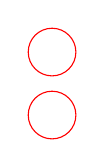
\begin{tikzpicture}
  \draw[red](0,0)circle(2ex);
  \draw[red](0,-0.8)circle(2ex);
\end{tikzpicture}
\caption{}
\label{fig:sfig0}
\end{subfigure}%
\begin{subfigure}{.24\textwidth}
\centering
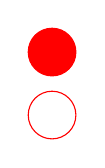
\begin{tikzpicture}
  \draw[red, fill=red](0,0)circle(2ex);
  \draw[red](0,-0.8)circle(2ex);
  \end{tikzpicture}
  \caption{}
  \label{fig:sfig1}
\end{subfigure}
\begin{subfigure}{.24\textwidth}
\centering
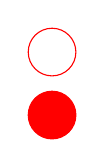
\begin{tikzpicture}
  \draw[red](0,0)circle(2ex);
  \draw[red, fill=red](0,-0.8)circle(2ex);
  \end{tikzpicture}
  \caption{}
  \label{fig:sfig2}
\end{subfigure}
\begin{subfigure}{.24\textwidth}
\centering
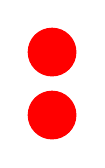
\begin{tikzpicture}
  \draw[red,fill=red](0,0)circle(2ex);
  \draw[red,fill=red](0,-0.8)circle(2ex);
  \end{tikzpicture}
  \caption{}
  \label{fig:sfig3}
\end{subfigure}
\caption{Methylation states; each figure shows a CpG/CpG-dyad on the parental and the daughter strand; each circle represents one CpG; plane red circles are methylated CpGs; (a) unmehtylated, (b) hemimethylated (upper strand unmethylated, lower strand methylated), (c) hemimethylated (vice versa), (d) fully methylated CpGs.}
\label{fig:methylationpatterns}
\end{figure}

The most common DNA modification is the addition of one methyl group to the fifth position in the cytosine ring of DNA. Methylation occurs mainly at \acfp{CpG}, where a cytosine nucleotide (C) is followed by a guanine nucleotide (G) in the DNA sequence. By the complementary basepairing of a \ac{CpG} to a \ac{GpC} on the other strand, there result two possible methylation positions at this CpG/CpG dyad. Hence, four methylation states may be discriminated. Either the dyad is unmethylated, fully methylated or one of the two cytosines is methylated and thus the dyad is hemimethylated. Figure \ref{fig:methylationpatterns} shows the possible methylation states. By the sequence of methylations over the whole genome, an individual methylation pattern can be retrieved for each organism\cite{DNAMethylation}.\\

\begin{figure}[h]
\centering
C\textcolor{red}{CG}AA\textcolor{red}{CG}T\textcolor{red}{CGCGCG}TCA\\
G\textcolor{red}{GC}TT\textcolor{red}{GC}A\textcolor{red}{GCGCGC}AGT
\label{CGI}
\caption{CpG-island with increased cytosine and guanine frequency; CpGs are marked in red.}
\end{figure}

Whereas the majority of \acp{CpG} in mammals are methylated, so called \acfp{CGI} are rather unmethylated. A \ac{CGI} is defined as region in the genome, where the frequency of \acp{CpG} is very high. Figure \ref{CGI} shows an example. The \acp{CGI} are associated to gene regulation as they are often located at the promoter region of genes. Hereby, cytosine methylation inhibits the gene expression; leading to changes in the methylation pattern of the DNA are effecting diseases like cancer\cite{Handbook}. Hypomethylation of repepetetive elements for example results in an unstable DNA and may increase the risk of cancer; as also the hypermethylation of cancer suppressor genes.\cite{DNAMethylation} Finally, DNA methylation is responsible for genomic imprinting and X-chromosome inactivation, whereby one of the two alleles respectively is transcribed and the other inactivated by methylation. Dysregulation may contribute to diseases like Prader-Willi syndrome, Angelman syndrome and cancer\cite{Walter}.\\

To detect methylcytosine, the most popular method is bisulfite sequencing, incorporated with \ac{PCR}. During bisulfite treatment, unmethylated cytosines are transformed to uracil, whereas methylated ones stay unaffected. \ac{PCR} sequencing is used to retrieve the base sequence\cite{Bisseq}. Nevertheless, bisulfite sequencing has multiple drawbacks. First, it depends on the correct conversion of cytosines to uracil, which is not given as errors during the bisulfite treatment may occur. Second, a differentiation  of \acf{5mC} and \ac{5hmC} is not possible because the two molecules respond in the same way to bisulfite treatment\cite{5hmC}. \ac{5hmC} is another DNA modification, which is associated to the process of active and passive demethylation\cite{demethyl}\cite{Giehr}. See section \ref{section:RelWork} for further details.\\

The transfer of the methyl group to the DNA is performed by \acfp{DNMT}. Five different \acp{DNMT} are distinguished in mammals: DNMT1, DNMT2, DNMT3A, DNMT3B and DNMT3L\cite{DNAMethylation}.\\
DNMT1 is commonly associated to maintanance methylation and the DNA replication process. Thereby, not only the DNA of the cell is transmitted from one cell generation to another, but also the methylation patterns. It is supposed, that DNMT1 has a preference for hemimythelated DNA. Subsequently, DNMT1 transfers the methylation by methylating the positions on the daughter strand that are methylated at the same position on the parental strand\cite{DNAMethylation}.\newline
DNMT2 is negligible if human DNA methylation is considered, because it methylates small RNA at the anticodon loop\cite{DNMT2}.\newline
DNMT3A and DNMT3B are de novo methyltransferases, which work during the early embryonic development to synthesize new methylations. Hereby, the common assumption is, that the enzymes do not show any preference neither for hemi- or unmethylated DNA nor for a DNA-strand. In other words, DNMT3A/B may add a methyl-group to any non-methylated \ac{CpG} at any DNA-strand. DNMT3L does not catabolize methylation, but increases the binding ability of DNMT3A/B and thus is required for establishing genomic imprinting\cite{DNAMethylation}.\newline
The loss of one of the methyltransferases leads to embryonic lethality\cite{DNAMethylation}.\newline
For simplification, DNMT3A and DNMT3B will not be further distinguished and called DNMT3.\\

So far a lot is known about the function of \acp{DNMT}, but some properties still remain unexplained:
\begin{itemize}
\item Why and where do the \acp{DNMT} bind?
\item On which conditions does the methylation event depend?
\item Which enzymes are able to methylate multiple \acp{CpG} in a row without disassociating from the DNA?
\item How much de novo and maintenance methylation do DNMT1 and DNMT3A/B perform?
\end{itemize}

To study the function of \acp{DNMT}, a computational, stochastic model is designed and fitted using real biological data.

\section{Foundations of statistics} 
\label{section:statistics}
Statistics is a mathematical field, dealing with the development of hypotheses, analysis and organization of empirical data. Here, the data are observations of real experiments, often called the sample data. The denotation sample space $\Omega$ refers to the collection of possible outcomes of the experiment\cite{Philosophy}. Two fields of statistics are distinguishable: descriptive and inferential statistics. Where descriptive statistics summarizes the data without changing it, using statistical methods like mean and standard deviation, inferential statistics is more about analysing data and making predictions based on probability theory\cite{Introduction}.\\
\newtheorem{definition}{Definition}
\begin{definition}[Probability]
The probability $P$ of an event $A$ is the likelihood of an event to happen. $P(A)$ can take any value between zero and one, where zero describes the impossibility and one the certainty of the event to occur\cite{BayStat}.
\end{definition}
\begin{definition}[Conditional Probability]
The conditional probability is the probability of an event to happen, given some prior knowledge $B$:\\
\begin{center}
$P(A \mid B) := \frac{P(A \cap B)}{P(B)}$ if $P(B) \neq 0$\cite{BayStat}.
\end{center}
\end{definition}
\begin{definition}[Independence]
Two events $A$ and $B$ are independent if $P(A \cap B) = P(A)P(B)$. Which may be written as $P(A\mid B) = \frac{P(A \cap B)}{P(B)} = P(A)$, so if the probability of A does not change compared to the probability of $A$ given $B$\cite{Probability}.
\end{definition}
\begin{definition}[Random Variable (RV)]
A random variable $X$ describes an outcome of an experiment. $X$ is defined as function $X : \Omega \rightarrow \mathbb{R}$\cite{ProbTheo}.
\end{definition}
Subsequently, we will focus on discrete \acp{RV}, which are a finite set of natural numbers.
\begin{definition}[Probability Distribution]
The representation of the probability of each value of a \ac{RV} is called a probability distribution\cite{ProbDistri}.
\end{definition}
\begin{definition}[Expectation]
$E(X) = \sum_{x \in X(\Omega)}{x \times P(x)}$ is the expected value of a discrete \ac{RV}. It may be seen as probability-weighted average of $\Omega$\cite{Probability}.
\end{definition}
\begin{definition}[Variance]
is the squared deviation from the mean. $V(X) = = \sum_{x \in X(\Omega)}{(x-E(X))^2 \times P(x)}$\cite{Probability}
\end{definition}
\begin{definition}[Covariance]
$Cov(X,Y) = E((X-E(X))(Y-E(Y)) = E(XY)-E(X)E(Y)$ is the covariance between two \acp{RV} $X$ and $Y$. If the value of the covariance is positive, there is a linear relationship between the two variables, otherwise, if the covariance is negative, the variables show opposite behaviour. Finally, the covariance is equal to zero if the variables are uncorrelated\cite{ProbDistri}.
\end{definition}
Given the definitions one to eight, the data can be described using a stochastic model.\\

\section{Markov models} 
\label{section:MM}
A discrete-time Markov model is a stochastic model that fulfils the Markov property. If the next state can only be determined by the current state and not by the previous one, a chain holds the Markov property, also called memoryless property\cite{Probability}:
\begin{equation}
P(X_n = x_n \mid X_{n-1} = x_{n-1}, ..., X_0 = x_0) = P(X_n = x_n \mid X_{n-1} = x_{n-1})
\end{equation}
Markov models can be used to describe a process and its development over time.\\

A \textbf{Markov chain} is the simplest Markov model. Named after Andrey Markov, the first paper about this model was published in 1906\cite{Markov}. This chain is a sequence of variables $X_1, X_2, ...$ whose outcomes are random, so called \acfp{RV}. Each \ac{RV} has a number of possible outcomes, the state space. Given a set of states $S = \{s_1, ..., s_n\}$ with transitions between the states, $p_{ij}$ is the transition probability from $s_i$ to $s_j$. And P of size $|S|\cdot|S|$ is the transition matrix containing the transition probabilities between all possible combinations of states.\newline
Let $\pi_0$ be the initial distribution of the chain $X$ s.t.\newline
\[\sum_{x \in \pi_0}{x} = 1,\]\newline
then\newline
\[\pi_1 = \pi_0 \cdot P\]\newline
is the distribution of $X$ at time $t=1$. We call $\pi$ the equilibrium distribution; the distribution of X that does not change from one time step to another or formally:\newline
$\pi = \pi \cdot P$.\\
In general, we distinguish between \acp{CTMC}, which act in continuous time and \acp{DTMC} in discrete time.\newline
Markov chains are the most used statistical model for many different real-world processes like for example PageRank\cite{MC}.\\
TODO: Ergodicity...?\\
\textbf{\acp{HMM}} are an extension of Markov chains and may also be interpreted as simple Bayesian network. There are two kinds of states in this model; hidden states S and observable output states O. Similarly, there is a transition probability matrix between the states in S and a matrix of output probabilities B between the hidden and the output states. Figure \ref{HMM} shows a graphic representation of an \ac{HMM}.\newline
This model is used, when there is information about the output of a process, but no knowledge about the states of the system.\\
\begin{figure}[h]
\centering
\begin{tikzpicture}[node distance=2cm,>=stealth',bend angle=45,auto,->,shorten >=1pt]
  \tikzstyle{place}=[circle,thick,draw=blue!75,fill=blue!20,minimum size=6mm]
  \tikzstyle{red place}=[place,draw=red!75,fill=red!20]
  	\node [place](S00){S00};
    \node [place](S01)[right of=S00]{S01};
    \node [place](S02)[right of=S01]{S02};
    \node [place](S03)[right of=S02]{S03};
    \node [place](S10)[below of=S00]{S10};
    \node [place](S11)[below of=S01]{S11};
    \node [place](S12)[below of=S02]{S12};
    \node [place](S13)[below of=S03]{S13};
    \node [red place](O0)[below of=S10]{O0};
    \node [red place](O1)[below of=S11]{O1};
	\node [red place](O2)[below of=S12]{O2};
	\node [red place](O3)[below of=S13]{O3};
	\path (S00)edge(S01)
    		   edge(S10)
    		   edge(S11)
    		   edge[bend right](O0)
    	  (S01)edge(S02)
    		   edge(S11)
    		   edge(S12)
    		   edge[bend right](O1)
    	  (S02)edge(S03)
    		   edge(S12)
    		   edge(S13)
    		   edge[bend right](O2)
    	  (S03)edge(S13)
    		   edge[bend right](O3)
    	  (S10)edge(S11)
    		   edge(O0)
    	  (S11)edge(S12)
    		   edge(O1)
    	  (S12)edge(S13)
    		   edge(O2)
    	  (S13)edge(O3);
\end{tikzpicture}
\caption{An HMM with eight hidden states(blue) and four emission states(red).}
\label{HMM}
\end{figure}

\section{Bayesian statistics} 
\label{section:Baystat}
By analysing observed data, one is able to develop a stochastic model which represents the process that generated the observed data. Utilizing Bayesian statistical methods, the parameters of the statistical model can be determined. Thereby, Bayesian statistics make use of the Bayes' theorem\cite{BayStat}.\newline
\begin{definition}[Bayes' Theorem]
Given two events $A$ and $B$ with $P(B) \neq 0$, the conditional probability of the events is given as\\
\centering{$P(A \mid B) = \frac{P(B \mid A) P(A)}{P(B)}$.}
\end{definition}
Here, $P(A)$ is the prior probability of $A$, so our expectation about the process without the knowledge of additional information. $P(A \mid B)$ is called the posterior probability, the probability of $A$, taking $B$ into account. Finally, $P(B \mid A)$ is the likelihood function; the probability of $B$, given that $A$ is true.\newline
The likelihood is an important function in Bayesian statistics. By maximizing the likelihood function, the most probable parameter of a model given an observation are decided. The likelihood function, it is defined as 
\begin{equation}
L(\Theta \mid x_0,...,x_n) = P_{\Theta}(x_0) ... P_{\Theta}(x_1).
\end{equation}
The process of determining the parameter $\Theta$ that maximizes the likelihood function given the data ${x_0,...,x_n}$ is called \textbf{\acf{MLE}}.\\

In the following, we describe the two major techniques in Bayesian statistics; \acf{MCMC} and \acf{ABC}.\\

The term \textbf{\ac{MCMC}} describes a collection of algorithms which simulate the distribution of a Markov chain after some time t. Once, the initial distribution $X_0$ and the transition matrix P are known, the simulation works by sampling from these distributions. Therefore, a random number is generated and based on the number, the state of the chain is identified, depending on in which range of the distribution the value is falling.\newline
E.g. assuming, we have three dice, two dice are biased and one regular. We want to compute the probability of throwing six pips. We choose randomly between the biased and the regular dice. The probability distribution of dice selecting is defined by $X_0$; the probability to dice six pips can be retrieved by considering the transition matrix $P$.
%\begin{figure}[h]
\begin{center}
%\centering
\begin{large}
$X_0$ =
\end{large}
$\begin{blockarray}{cccc}
  & dice 1 & dice 2 & dice 3 \\
  \begin{block}{c[ccc]}
    & 1/3 & 1/3 & 1/3 \\
  \end{block}
\end{blockarray}$
%\caption{initial distribution $X_0$}
%\end{figure}
%\begin{figure}[h]
%\centering
\\
\begin{LARGE}
P =
\end{LARGE}
$\begin{blockarray}{ccccccc}
  & 1 & 2 & 3 & 4 & 5 & 6 \\
  \begin{block}{c[cccccc]}
    dice 1 & 2/15 & 2/15 & 2/15 & 2/15 & 2/15 & 1/3 \\
    dice 2 & 1/3 & 1/12 & 1/12 & 1/12 & 1/6 & 1/4 \\
    dice 3 & 1/6 & 1/6 & 1/6 & 1/6 & 1/6 & 1/6 \\
  \end{block}
\end{blockarray}$
%\caption{transition matrix P}
%\end{figure}
\end{center}

\begin{algorithm}
\begin{algorithmic}
\State $r \gets random(0,1)$
\For {$i \in len(X_0)$}
\If {$r \leq X_0[i]$}
\State $dice \gets i$
\State break
\Else
\State $r \gets r - X_0[i]$
\EndIf
\EndFor
\State $r \gets random(0,1)$
\For {$i \in len(P[dice])$}
\If {$r \leq P[dice][i]$}
\State $pips \gets i$
\State break
\Else
\State $r \gets r - P[dice][i]$
\EndIf
\EndFor
\end{algorithmic}
\caption{\label{MCMC} a Markov Chain Monte Carlo simulation}
\end{algorithm}

The simulation starts by generating the first random number between zero and one. If the value falls into the first interval of $X_0$, we choose the first dice. Otherwise, if the value is greater than 1/3, but smaller than 2/3, so if the value falls in the second interval, we choose the second dice. If that also does not hold, we select dice three.\newline
After initializing the dice, the rolling of the dice is simulated by generating random variates again. The row, which represents the selected dice, gives the probability distribution of pips. If we roll dice one or two, the probability of throwing six pips is higher than if we rolled dice three. By repeating the simulation multiple times, we get a specific distribution of pips for each combination of selected dice. Comparing a real experiment with multiple throws to our simulated distribution, we are able to predict the dice used in the experiment. Figure \ref{MCMC} shows the pseudo-code of one simulation run of an MCMC.\\

TODO:forward-backward algorithm?\\

\begin{algorithm}
\begin{algorithmic}
\State $sim \gets prior()$
\If {$dist(sim,data) < \epsilon$}
\State accept sim
\Else
\State reject sim
\EndIf
\end{algorithmic}
\caption{\label{ABC} Approximative Bayesian Computation}
\end{algorithm}

A second method in computer simulations is \textbf{\acf{ABC}}. In contrast to \ac{MCMC}, \ac{ABC} does not need to evaluate the likelihood function, which may be an advantage because the evaluation is computational costly and sometimes not possible. Instead, the similarity of the observed to the real data is measured with a distance function. Hereby, samples are drawn from the prior distribution. If the distance of the sample to the desired value is greater than a threshold $\epsilon$, the sample is rejected, otherwise it is accepted. The posterior distribution results from the set of accepted samples (see figure \ref{ABC} for the pseudo-code)\cite{ABC}.

\section{Problem} 
\label{section:Problem}
As mentioned in section \ref{section:DNAMeth}, our general goal is to study the function of \acp{DNMT}, especially to determine the conditions for methylation activity. We are given the methylation patterns of multiple samples and loci, derived from biological experiments and bisulfite sequencing. For each loci and individual the methylation patterns are known before and after a specific number of replications. These methylation patterns form a distribution, called the methylation pattern distribution. We use Markov models and the given data to model the function of \acp{DNMT} and to predict their behaviour. Each state represents the methylation state of one dyad. Formally,
\begin{align}
S_i := \text{methylation state of CpG-dyad i}\\
S_i = \left\{
\begin{array}{l}
\text{unmethylated} \\
\text{hemimethylated} \\
\text{methylated.}
\end{array}
\right.\newline
\end{align}
Let $X$ be the desired Markov chain and $X_0$ be the given initial distribution of $X$. Further, let $P$ be the transition matrix between the states:\newline
$P$ := methylation probabilities\newline
We want to compute $P$, such that the distribution of our simulation of the Markov model after n time-steps is as similar as possible to the known distribution $X_n$.\\

\textbf{\textsc{Problem:}} Inference of parameters for DNA methyltransferase\newline
\textbf{Given:} initial pattern distribution $X_0$, pattern distribution at time $n$ $X_n$\newline
\textbf{Goal:} determine transition matrix $P$\\

%In the context of \acp{DNMT}, Markov models are used to simulate the function of these enzymes, making use of results from biological experiments. Here, few is known about the properties of methyltransferases. Under which condition does the enzyme bind to the DNA and when does it methylate? But the methylation patterns before and after the catabolism of the \acp{DNMT} are known. From the methylation pattern distribution, a sequence of methylation states can be retrieved. Each methylation (unmethylated, hemimethylated, methylated) of one \ac{CpG}-dyad is an output state, whereas the binding state and methylation conditions of the \ac{DNMT} at each \ac{CpG} are hidden states. Thus the traversing probabilities between the hidden states P are equal to the probabilities of the \acp{DNMT} to bind/fall of and the output probabilities represent the different methylation probabilities.\\
%Given the output sequence\newline
%\begin{align}
%O_i := \text{methylation state of CpG-dyad i}\\
%O_i = \left\{
%\begin{array}{l}
%\text{unmethylated} \\
%\text{hemimethylated} \\
%\text{methylated,}
%\end{array}
%\right.\newline
%\end{align}
%we are able to determine the most likely sequence of S\newline
%$S_i := \text{state of DNMT at CpG i}$\newline
%Moreover, P and B can be reconstructed by computer simulation of the \ac{DTMC}.
%Moreover, our goal is to determine\newline
%\begin{align}
%P := \text{probability of DNMT to change binding state}\\
%B := \text{methylation probabilities.}
%\end{align}

Recently, different models and computational approaches were studied in order to predict the methylation process. Here we present some of them.\\

\section{Related work} 
\label{section:RelWork}
One example of such a model to study the methylation activity of \ac{DNMT} was introduced by \textbf{Genereaux et al.}\cite{Genereaux} in 2005. Using bisulfite \ac{PCR} newly synthesized methylations on both strands were discovered, which cannot both result from the malfunction of maintenance methylation. Maintenance methylation occurs only on the daughter strand and independent of which strand is the daughter strand, the origin of the methylation of the other strand is unclear. Thus, the authors assume that de novo methylation exists and develop a model, where $\mu$ represents the maintenance methylation rate and $\delta_p$ and $\delta_d$ the de novo methylation rate at the parent and daughter strand respectively. The methylation state of each \ac{CpG}-dyad is either $M$, $H$ or $U$ (methylated, hemimethylated, unmethylated), whereas the state of a single \ac{CpG} is either m (methylated) or u (unmethylated). Given the methylation rates, the methylation state at time t can be rewritten depending on the previous state like in equations \ref{M}-\ref{U}.
\begin{align}
M_t &= \mu m_{t-1} + \delta_d \delta_p u_{t-1},\label{M}\\
H_t &= \delta_d (1- \delta_p) u_{t-1} + \delta_p (1- \delta_d) u_{t-1} + (1-\mu) m_{t-1},\\
U_t &= (1- \delta_p) (1- \delta_d) u_{t-1},\label{U}
\end{align}
where $(1-x)$ is the rate of a specific methylation not happening.\newline
By rewriting the equations above, an equations for the equilibrium distribution of the methylation states can be retrieved. Additionally, the likelihood of the states can be computed given the methylation rates.\\

\textbf{Fu et al.(2010)}\cite{errors} used the same model and data from double-stranded DNA to infer the methylation parameters, considering errors in the methylation measuring process. These errors may occur during bisulfite conversion. Regularly, unmethylated cytosines are converted to uracil and methylated cytosines recognized. In the opposite case, unmethylated cytosines are not converted or methylated cytosines falsely converted. The experiments supports the assumption that de novo methylation occurs on both strands. Moreover, the authors come to the conclusion that the methylation rates do not follow their prior distribution, but seems to be location dependant.\\

Another approach which includes bisulfite conversion errors in the model was introduced by \textbf{Arand et al.}\cite{Wolf}. They developed a \ac{HMM} similar to \ac{DTMC} proposed by Sontag, Lorincz and Luebeck\cite{Sontag}. The transition matrix of the Markov Chain is composed of three transition matrices; one represents the de novo probability, one the maintenance probability and one the strand segregation probabilities. Based on this model, the equilibrium distribution and the methylation level depending on the methylation probability can be computed. Contrary to Sontag, Lorincz and Luebeck, Arand et al. did not compute the maximal methylation probabilities, but the methylation rates and the influence of bisulfite conversion errors using a maximum likelihood approach.\\

Recently, \textbf{Giehr et al.}\cite{Giehr} developed a similar \ac{HMM}, which also includes the hydroxylation probability. In the paper the authors distinguish between the occurrence of \ac{5mC} and \ac{5hmC} and compute their distribution by making use of oxidative bisulfite sequencing. This differentiation was not possible before, using \ac{BS-seq}. Here, a \ac{HMM} was used with three transition matrices considering the cell division, methylation and hydroxylation probabilities. The observable states of the model are the methylation patterns after the full replication process, whereas the hidden states are the states between single transitions. The parameters estimated using \ac{MLE} suppose that \ac{5hmC} contributes significantly to the demthylation process and that the hydroxylation and methylation level at the loci decreases along the DNA and thus seems to be location-dependant.\\

The first of three approaches below, covering not only a single \ac{CpG} at a time for the computation of the methylation parameter, is by \textbf{Fu et al. (2012)}\cite{Fu}. Based on earlier suppositions that the methylation probabilities may rely on neighbouring methylation states, they developed their model to study the processivity of \acp{DNMT}. They call an enzyme to work processively if it methylates multiple \acp{CpG} in a row without dissociating from the DNA. In total, the model uses four parameter:
\begin{align*}
\rho := \text{probability of DNMT to fall off from DNA (dissociation probability)}\\
\tau := \text{probability of DNMT to bind to DNA (association probability)}\\
\mu := \text{probability to methylate hemimethylated CpG/CpG-dyad}\notag\\
		\text{(maintenance methylation probability)}\\
\delta := \text{probability to methylate unmethylated CpG/CpG-dyad}\notag\\
		\text{(de novo methylation probability.)}
\label{parameters}
\end{align*}
Here, $\rho = 0$ means the enzyme is highly processive, which means it continues its work from one \ac{bp} to another without unbinding. Otherwise, the enzyme can dissociate from the previous \ac{bp} and bind again at any following \ac{bp}. The next binding location may be multiple \acp{bp} apart but may also be the direct neighbour of the position, where the enzyme dissociated. A situation, where the methyltransferase is bound to the DNA at a specific \ac{bp} and the following \ac{bp}, may be caused by one of the following events:
\begin{enumerate}
\item \ac{DNMT} works processively (probability $1-\rho$)
\item \ac{DNMT} dissociates but reassociates at next \ac{bp} (probability $\rho * \tau$)
\end{enumerate}
The four parameter are identified for DNMT1, DNMT3A and DNMT3B respectively using the forward-backward algorithm for \acp{MCMC} (see section \ref{section:Baystat} for forward-backward algorithm). It is therefore assumed, that DNMT1 works on the daughter strand and DNMT3A/B on the parental as also on the daughter strand.\newline
Additionally included in the model are bisulfite conversion error rates as described in earlier approaches.\newline
In the paper, double-stranded methylation patterns from three loci were used as output states of the \ac{HMM}. The goal was to assemble the sequence of hidden states, modelled as the association state of the \acp{DNMT}. Formally, $P(Q_{ij},D_{ij}\mid M_{ij},R_{ij}^P,R_{ij}^D)$ is computed, where $Q_{ij}$ and $D_{ij}$ are the methylation states of the parent and daughter strand after replication respectively and  $M_{ij},R_{ij}^P$ and $R_{ij}^D$ are the association states of DNMT1, DNMT3 at the parent and daughter strand. The full transition table holds 9x4 states and is a combination of the four parameters from \ref{parameters}.\newline
Two of the three loci used are inactive X (Xi)-linked, namely FMR1 and G6PD. The third locus, LEP, is located on Chromosome seven. In contrast to the autosomal locus, the x-chromosomal loci are highly methylated and consist of large blocks with hemimethylated dyads. The authors suppose that these blocks help to identify the emission probabilities, especially to differentiate between the processive behaviour of the methyltransferases and the dissociation-reassociation event. Consistent to this presumption, in the experiments DNMT1 seems to be highly processive at FMR1 and G6PD, whereas the association parameter are difficult to identify at LEP. Regarding the results of the methylation probabilities, the different loci are conform. DNMT1 performs nearly exclusively maintenance methylation, while no further knowledge may be received from the experiments regarding the methylation probabilities of DNMT3, because the considered confidence intervals of $\mu$ and $\delta$ are equal to the uniform prior. These results are retrieved by partially restricting the parameter space, which Fu et al. suppose in order to distinguish the activity of DNMT1 and DNMT3.\\

Based on the findings of Fu et al. (2012), \textbf{Bonello et al.}\cite{Bonello} focused on four models and evaluated their advantages and limitations.\newline
First, a location-dependant model was proposed, where the de novo methylation and demethylation rate decrease along the DNA-strand. The de novo methylation probability $\alpha$ and demethylation probability $\beta$ are defined as:
\begin{align}
\alpha_i = P(S_i[t] = 1 \mid S_i[t-1] = 0) = exp(-\lambda i),\\
\beta_i = P(S_i[t] = 0 \mid S_i[t-1] = 1) = exp(\gamma (i-13)),
\end{align}
where $S_i[t]$ is the methylation state of the dyad at position $i$ at time $t$ and $\lambda$ and $\gamma$ are the parameter of interest.\newline
The other three models are location- and neighbour-dependent and are modelled similar to the model from 2012:
\begin{equation}
P(S_i[t] = 1 \mid S_{i-1}[t] = 0, S_i[t-1] = 0) = 1-\psi_i (1-\beta_i).
\end{equation}
Here, $\psi_i$ is the probability that the methylation state at position $i-1$ is different than the one at position $i$. The three approaches M2, M3, M4 differ only in the way $\psi_i$ is defined.
\begin{align}
\psi_i = \psi\\
\psi_i = exp(-\rho i)\\
\psi_i = exp(\rho (i-13))
\end{align}
In other words, M2 represents a model, where $\psi$ shows no location dependence, and M3 and M4 location dependence following parameter $\rho$. No model was invented, where neither $\psi$ nor $\alpha$ and $\beta$ were location dependent as in Fu et al.(2012). The reason for this was, that, looking at the distribution of methylation over the DNA at the \ac{MGMT} promoter, the most methylations seem to be located at the first \acp{CpG} and the methylation rate increases towards the end of the promoter region.\newline
The different models were evaluated and the parameter estimated using \ac{ABC}. It was revealed that model two fitted the four samples from the promoter best. Thus, the methylation state at position i seems to dependent on the preceding methylation state at the whole locus of the same amount, whereas the methylation probability is not stationary over all \acp{CpG}\cite{Bonello}.\\

Finally, another idea of neighbour-dependant modelling is to examine not only the preceding \acp{CpG}, but to consider \ac{CpG}-triplets, so to determine methylation probabilities, depending on the methylation state of the preceding and succeeding \ac{CpG} (\textbf{L\"{u}ck et al.}\cite{Lueck}). Remembering that the DNA is double-stranded, each triplet has six possible methyl-binding positions. Because each of these positions may be methylated or unmethylated, there are $2^6 = 64$ possible methylation patterns for one triplet. Nevertheless, because for each triplet we consider only the change of methylation state of the dyad in the center, there exist only four possible transitions for maintenance and de novo methylation respectively; namely, either none of the neighbouring \acp{CpG}, the right neighbour, the left neighbour or both neighbours are methylated. The methylation state of the centered \ac{CpG} on the parent strand is deciding in case of maintenance methylation. No dependence is between the transition probabilities of the methylation patterns and the upper left and right position of the triplet. The approach also takes bisulfite conversion errors and a strand selection after replication into account.\newline
Four parameters are tracked in total: the maintenance methylation probability $\mu$, the dependency parameters for the left and right neighbour $\psi_L, \psi_R$ and the de novo methylation probability $\tau$. Hereby, the identification of the parameters is performed by \ac{MLE}. Thereby, the final parameters have the maximal probability to produce the same methylation pattern distribution as our data.\newline
As in \cite{Wolf}, three kind of \ac{BS-seq} data are used. Two of them are \ac{KO} data, where either DNMT1 or DNMT3A and DNMT3B are inactivated in the replication process (DNMT1KO, DNMT3A/BKO). The third is \ac{WT} data, where all enzymes are active.\newline
The results show independence of the succeeding \ac{CpG} for DNMT1 and DNMT3 and an indicate for a dependence of DNMT3 on the predecessor. Moreover, the dependence of the model on the order of \ac{DNMT} activity was studied. This means, it was tested if the results changed if the order of \acp{DNMT} varies or if the enzymes work alternating at one position compared to the whole strand. Concluding, that the order of DNMT1 and DNMT3A/B matters as the results are different if DNMT1 is not the first enzyme in \ac{WT}. But the order of DNMT3A and DNMT3B and of the alteration seems not to be significant.\\

In the following, we describe our model, which follows the approach of \cite{Fu}, introduced earlier. It will be shown that it is possible to distinguish the functions of DNMT1 and DNMT3 and that, using our model, we are able to endorse earlier assumptions about association and methylation rates. Moreover, we compare different computational approaches to estimate the process' parameters.